\section{Implementation}\label{planta:sec:implementation}

\acronym is implemented as a ROS~2-based system to facilitate its use in robotic applications. It integrates \plansys~\cite{plansys2} for planning and plan execution, System Modes~\cite{nordmannSystemModes2021} for managing system reconfiguration, and a custom ROS~2 package that implements the OWL to PDDL translation.

\subsection{\owltopddl tool}
To apply the OWL to PDDL translation, this work provides a standalone Kotlin-based executable that performs the translation independently of ROS~2. Additionally, a ROS~2 package is provided to integrate the tool with the ROS~2 ecosystem. While the transformation approach builds on prior work that translates OWL axioms into PDDL rules~\cite{DBLP:conf/aaai/Borgwardt0KKNS22}, existing tools are not well-suited for robotic self-adaptation. In particular, the \pddltomasys ontology includes numerical values that require translation, a feature unsupported by current tools. Additionally, developing a new tool allowed for optimizations, such as specifying the PDDL types of ontology instances. These types are exported to the PDDL domain model to help reduce planning time. Both the OWL to PDDL tool and the associated ROS~2 package are publicly available.\footnote{\url{https://github.com/remaro-network/dlToPlanning}}

\subsection{Planning and plan execution}\label{planta:sec:impl_plansys}

For planning and plan execution, this work leverages \plansys. However, since \plansys does not support all PDDL requirements imposed by the OWL to PDDL transformation step, this work extends \plansys to support existential preconditions (PDDL 1.1), derived predicates (PDDL 2.2), equality between non-numeric objects (e.g., $(\texttt{=}\; ?p\; \texttt{constant})$), negation of composite expressions (e.g., $(\texttt{not}\; (\texttt{=}\; ?a\; ?b))$), and the execution of non-durative actions.

This work uses the Fast Downward~\cite{helmert2006fast} planner for automated planning since it supports derived predicates and existential preconditions. To use Fast Downward with \plansys, this work implements a \plansys plugin for the Fast Downward planner, which is publicly available online\footnote{\url{https://github.com/kas-lab/downward_ros}}.

Adding support for derived predicates and existential preconditions in \plansys resulted in conceptual changes to the \emph{preconditions evaluation} and \emph{apply action effects} algorithms that are used in the plan execution process. Furthermore, it required the addition of a mechanism that is able to evaluate derived predicates at runtime to infer new predicates in a reasonable amount of time. The other extensions to \plansys aforementioned required only additional implementation.

The synthetic domain in \Cref{planta:lst:example_derived} is used throughout this section to keep the examples compact. The derived predicates that \owltopddl generates from the \pddltomasys ontology (\Cref{planta:sec:owl_to_pddl}) share its structure: they are defined over other derived predicates and use existential quantification and negation. Predicates such as \texttt{f\_active} and \texttt{fd\_realisability} are re-derived from base facts such as \texttt{functionGrounding} that the reconfiguration actions modify (\Cref{planta:sec:plan_transformation_taca}).

\paragraph{Preconditions evaluation algorithm}

In \plansys, the \emph{preconditions evaluation algorithm} $\texttt{Evaluate}(\pddlActPre_a, \pddlState)$ determines whether the preconditions $\pddlActPre_a$ of action $a \in \pddlActions$ are satisfied in a given state $\pddlState$. This algorithm is used both during plan graph construction~\cite{pddl_plans_bt} to build a behavior tree for plan execution,
and at runtime by the resulting plan graph BT to continuously verify the feasibility of executing actions. The current evaluation algorithm assumes that there are no free variables in the preconditions, i.e., all parameters are grounded with objects $o \in \pddlObjects$ during the planning process.

This assumption no longer holds when existential preconditions are introduced. For example, consider the plan $\pi = (\underline{a}_1)$ as a valid solution to a \emph{problem instance} $\pddlInstance$ of the \emph{planning domain} shown in~\Cref{planta:lst:example_derived}, where $name_{\underline{a}_1} = \texttt{action1}$ and $\pddlActParam_{\underline{a}_1} = (\texttt{instance1})$. In this case, the existential precondition introduces a free variable $?y$ that remains ungrounded at planning time.

Evaluating such preconditions requires checking whether there exists an object $o \in \pddlObjects$ such that the variable $?y$ can be unified with $o$, and the resulting grounded formula satisfies the logical condition defined in the precondition body. In the example, this corresponds to verifying whether there exists an object $o$ such that the atom $(\texttt{predicateAA}~\texttt{o})$ is contained in the current state $\pddlState$, e.g., $(\texttt{predicateAA}~\texttt{instance2}) \in \pddlState$.

With the addition of derived predicates, the evaluation algorithm is no longer limited to checking action preconditions, it must also evaluate the conditions of derived predicates, i.e., $\texttt{Evaluate}(C, \pddlState)$, where $C ::= \pddlActPre_a \mid \phi(\pddlActParam)$. In this setting, the evaluation of a precondition $c \in C$ cannot be performed by simply verifying whether it is satisfied in the current state $\pddlState$. Instead, the relevant derivation rules $r \in \pddlDerRules$ must be applied to the current state $\pddlState$ to determine whether the predicates $p \in c$ can be derived. For example, in the \emph{planning domain} shown in~\Cref{planta:lst:example_derived}, given a state $s = \{(\texttt{predicateA}~\texttt{instance1}), (\texttt{predicateAA}~\texttt{instance2})\}$, the precondition of $\texttt{action1}$ is satisfied only if the derived predicate $\texttt{(inferredA ?x)}$ (lines 1–2) is successfully inferred. To support the evaluation of existential preconditions and derived predicates in \plansys, this work proposes the evaluation algorithm described in \Cref{planta:S-alg:eval}.

\begin{figure}[tbp]
\centering
\begin{minipage}[t]{0.49\linewidth}
\begin{lstlisting}[language=PDDL, firstnumber=1, numbers=left, stepnumber=1, xleftmargin=2em]
(:derived (inferredA ?x)
  (predicateA ?x))
(:derived (inferredAA ?x)
  (inferredA ?x))
(:derived (inferredB ?x)
  (or (predicateB ?x)
      (inferredAB ?x)))
(:derived (inferredBB ?x)
  (inferredB ?x))
(:derived (inferredAB ?x)
  (or (inferredA ?x)
      (inferredB ?x)))
\end{lstlisting}
\end{minipage}
\hfill
\begin{minipage}[t]{0.49\linewidth}
\begin{lstlisting}[language=PDDL, firstnumber=13, numbers=left, stepnumber=1, xleftmargin=2em]
(:action action1
  :parameters (?x)
  :precondition (and (exists (?y)
    (and (predicateA ?x)
         (predicateAA ?y)
         (inferredA ?x))))
  :effect (and (predicateB ?x)))
(:action action2
  :parameters (?x)
  :precondition (and
    (inferredB ?x)
    (inferredAB ?x))
  :effect (and (predicateC ?x)))
\end{lstlisting}
\end{minipage}
\caption{PDDL example with derived predicates and existential preconditions.}%
\label{planta:lst:example_derived}
\Description{Two-column PDDL example. The left column defines five derived predicates.
\texttt{inferredA} depends on \texttt{predicateA}. \texttt{inferredAA} depends on
\texttt{inferredA}. \texttt{inferredB} depends on \texttt{predicateB} or
\texttt{inferredAB}. \texttt{inferredBB} depends on \texttt{inferredB}. Finally,
\texttt{inferredAB} depends on \texttt{inferredA} or \texttt{inferredB}. The right
column defines two actions. Action1 requires \texttt{predicateA} and \texttt{inferredA}
for its parameter and the existence of an object satisfying \texttt{predicateAA}, then
adds \texttt{predicateB}. Action2 requires \texttt{inferredB} and \texttt{inferredAB},
then adds \texttt{predicateC}.}
\end{figure}


\paragraph{Derived predicates resolution}

The derived predicate resolution implemented in this work adheres to the definition of derived predicates introduced by Thiébaux et al.~\cite{THIEBAUX200538}, which extends the original PDDL~2.2~\cite{edelkamp2004pddl2} specification. This definition allows derived predicates to depend on other derived predicates, including recursive self-dependencies, and allows negated derived predicates in their preconditions, provided that such negation does not occur within a recursive cycle.

To address this problem, this work proposes representing the derived predicates from a PDDL formulation as a directed graph. For example, the PDDL formulation described in \Cref{planta:lst:example_derived} can be represented as the graph depicted in \Cref{planta:fig:derived_graph}. In this graph, nodes in the upper layer (depth 0) represent predicates, functions, or instances, while nodes in the lower layers (depth one or more) represent derived predicates. The edges indicate dependencies between the nodes, with arrows pointing from parent to child nodes. For example, the edge from $\texttt{predicateA}$ to $\texttt{inferredA}$ indicates that the latter depends on the former.

\begin{figure}[tbp]
    \centering
    \begin{subfigure}[t]{0.48\linewidth}
        \vspace{0pt} % Aligns top
        \centering
        %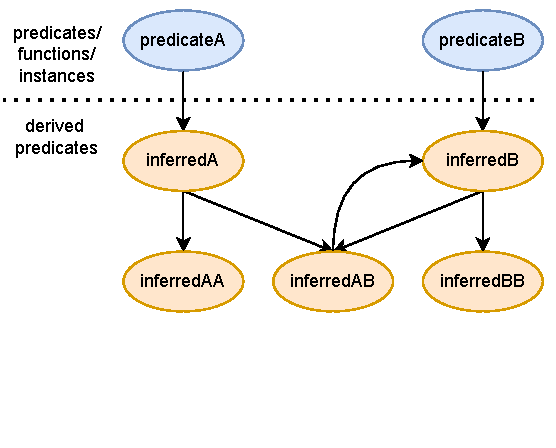
\includegraphics[width=\linewidth]{pddl/figures/derived_graph.pdf}
        \resizebox{\linewidth}{!}{\begin{tikzpicture}[font=\sffamily]
    
    \coordinate (origin) at (0,0);
    \draw (origin) node[bubbleBlue] (predicateA) {predicateA\strut};
    
    \draw ($(predicateA) + (5,0)$) node[bubbleBlue] (predicateB) {predicateB\strut};
    
    \draw ($(predicateA) + (0,-1.7)$) node[bubbleGreen] (inferredA) {inferredA\strut};
    \draw ($(predicateB) + (0,-1.7)$) node[bubbleGreen] (inferredB) {inferredB\strut};
    
    \draw ($(inferredA) + (0,-1.5)$) node[bubbleGreen] (inferredAA) {inferredAA\strut};
    \draw ($(inferredA) + (2.5,-1.5)$) node[bubbleGreen] (inferredAB) {inferredAB\strut};
    \draw ($(inferredB) + (0,-1.5)$) node[bubbleGreen] (inferredBB) {inferredBB\strut};
    
    \phantom{\draw ($(inferredAA) + (0,-1.7)$) node[bubblePurple] (action1) {action1\strut};} % phantom for alignment with other figure
    
    \draw[arrow] (predicateA) -- (inferredA);
    \draw[arrow] (predicateB) -- (inferredB);
    
    \draw[arrow] (inferredA) -- (inferredAA);
    \draw[arrow] (inferredA) -- (inferredAB);
    \draw[arrow] (inferredB) -- (inferredAB);
    \draw[arrow] (inferredB) -- (inferredBB);
    
    \draw[arrow] (inferredAB) to [bend left] (inferredB);
    
    % labels
    \draw ($(predicateA) + (-2.2,0)$) node (topLabel) {\begin{tabular}{c}
            predicates/\\
            functions/\\
            instances
    \end{tabular}};

    \draw ($(topLabel) + (0,-1.2)$) node (botLabel) {\begin{tabular}{c}
            derived\\
            predicates
    \end{tabular}};
    
    % dotted line
    \draw[loosely dotted,
        draw=black, 
        line width=1.5pt] ($(topLabel) + (-0.7,-0.7)$) -- ++ (9,0);
    
    
\end{tikzpicture}}
        \caption{Complete graph.}%
        \label{planta:fig:derived_graph}
    \end{subfigure}
    \hfill
    \begin{subfigure}[t]{0.48\linewidth}
        \vspace{0pt} % Aligns top
        \centering
        %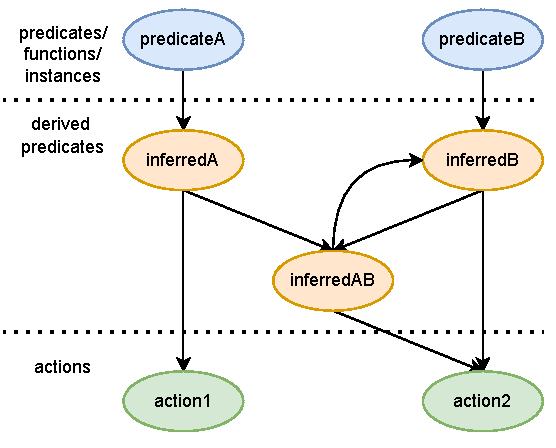
\includegraphics[width=\linewidth]{pddl/figures/derived_graph_pruned.pdf}
        \resizebox{\linewidth}{!}{\begin{tikzpicture}[font=\sffamily]
    
    \coordinate (origin) at (0,0);
    \draw (origin) node[bubbleBlue] (predicateA) {predicateA\strut};
    
    \draw ($(predicateA) + (5,0)$) node[bubbleBlue] (predicateB) {predicateB\strut};
    
    \draw ($(predicateA) + (0,-1.7)$) node[bubbleGreen] (inferredA) {inferredA\strut};
    \draw ($(predicateB) + (0,-1.7)$) node[bubbleGreen] (inferredB) {inferredB\strut};
    
    \draw ($(inferredA) + (0,-1.5)$) node (inferredAA) {};
    \draw ($(inferredA) + (2.5,-1.5)$) node[bubbleGreen] (inferredAB) {inferredAB\strut};
    \draw ($(inferredB) + (0,-1.5)$) node (inferredBB) {};
    
    \draw ($(inferredAA) + (0,-1.7)$) node[bubblePurple] (action1) {action1\strut};
    \draw ($(inferredBB) + (0,-1.7)$) node[bubblePurple] (action2) {action2\strut};
    
    
    \draw[arrow] (predicateA) -- (inferredA);
    \draw[arrow] (predicateB) -- (inferredB);
    
    \draw[arrow] (inferredA) -- (action1);
    \draw[arrow] (inferredA) -- (inferredAB);
    \draw[arrow] (inferredB) -- (inferredAB);
    \draw[arrow] (inferredB) -- (action2);
    \draw[arrow] (inferredAB) -- (action2);
    
    \draw[arrow] (inferredAB) to [bend left] (inferredB);
    
    % labels
    \draw ($(predicateA) + (-2.2,0)$) node (topLabel) {\begin{tabular}{c}
            predicates/\\
            functions/\\
            instances
    \end{tabular}};

    \draw ($(topLabel) + (0,-1.2)$) node (midLabel) {\begin{tabular}{c}
            derived\\
            predicates
    \end{tabular}};

    \draw ($(topLabel) + (0,-4.5)$) node (botLabel) {\begin{tabular}{c}
            actions
    \end{tabular}};
    
    % dotted line
    \draw[loosely dotted,
        draw=black, 
        line width=1.5pt] ($(topLabel) + (-0.7,-0.7)$) -- ++ (9,0);
        
   \draw[loosely dotted,
   draw=black, 
   line width=1.5pt] ($(botLabel) + (-0.7,0.5)$) -- ++ (9,0);
    
    
\end{tikzpicture}}
        \caption{Pruned graph for $\pi=(\texttt{action1}, \texttt{action2})$.}%
        \label{planta:fig:pruned_graph}
    \end{subfigure}
    \caption{Derived predicates resolution graphs for the PDDL formulation in \Cref{planta:lst:example_derived}: (a) the full dependency graph and (b) the pruned graph for the plan $\pi = (\texttt{action1}, \texttt{action2})$. The predicates $\texttt{predicateAA}$ and $\texttt{predicateC}$ are omitted to simplify the visualization, as they are not relevant to the graph structure due to having no child predicates.}%
    \label{planta:fig:derived_graphs_combined}
\Description{Two directed dependency graphs, with arrows pointing from a predicate to predicates or
actions that depend on it. In the complete graph on the left, \texttt{predicateA} leads
to \texttt{inferredA}, which leads to \texttt{inferredAA} and \texttt{inferredAB}.
PredicateB leads to \texttt{inferredB}, which leads to \texttt{inferredAB} and
\texttt{inferredBB}. InferredAB also points back to \texttt{inferredB}, forming a cycle.
In the pruned graph on the right, \texttt{inferredAA} and \texttt{inferredBB} are
removed. \texttt{action1} depends on \texttt{inferredA}, and \texttt{action2} depends on
\texttt{inferredB} and \texttt{inferredAB}. The cycle is retained.}
\end{figure}

To solve derived predicates, this work introduces \Cref{planta:S-alg:solve_derived}. It partitions the resolution graph into strongly connected components~(SCCs) using Tarjan's algorithm~\cite{doi:10.1137/0201010}, which separates acyclic from cyclic components. The acyclic components are resolved in topological order, while the cyclic components are resolved using a fixed-point iteration. Root nodes are considered solved by definition, as they correspond to non-derived predicates. For instance, in the graph shown in \Cref{planta:fig:derived_graph}, the derived predicates $\texttt{inferredB}$ and $\texttt{inferredAB}$ form a cycle, whereas the other derived predicates are acyclic.

\paragraph{Apply action effects algorithm}

With the addition of derived predicates, applying an action's effects can invalidate previously derived predicates and make new ones derivable. Instead of recomputing all derived predicates, this work exploits the structure of the derived predicates graph to re-evaluate only the derived predicates that depend on the predicates modified by the effects (\Cref{planta:S-alg:apply_new}). For example, in the PDDL domain described in \Cref{planta:lst:example_derived}, applying the action $(\texttt{action1}~\texttt{instance1})$ adds $(\texttt{predicateB}~\texttt{instance1})$ to the state, which requires re-evaluating only the derived predicates $\texttt{inferredB}$, $\texttt{inferredAB}$, and $\texttt{inferredBB}$.

\paragraph{Derived graph pruning by action}

To optimize the evaluation of derived predicates during plan graph generation and runtime execution in \plansys, this work proposes appending the actions defined in the \emph{planning domain} to the derived graph and pruning it to retain only the predicates relevant to the current action plan. For example, given the \emph{planning domain} in \Cref{planta:lst:example_derived} and the plan \(\pi = (\texttt{action1}, \texttt{action2})\), the derived graph shown in \Cref{planta:fig:derived_graph} can be pruned to the graph in \Cref{planta:fig:pruned_graph}, avoiding the unnecessary resolution of predicates \(\texttt{inferredAA}\) and \(\texttt{inferredBB}\).


%%% Local Variables:
%%% mode: latex
%%% TeX-master: "main"
%%% End:
